\section{Comparison of 3 Computer Vision Models}
\label{sxn:cv}

\paragraph{Empirical Metrics vs Test Accuracies for CV models}

\begin{figure}[t]
    \centering
    \subfigure[ Frobenius Norm ]{
        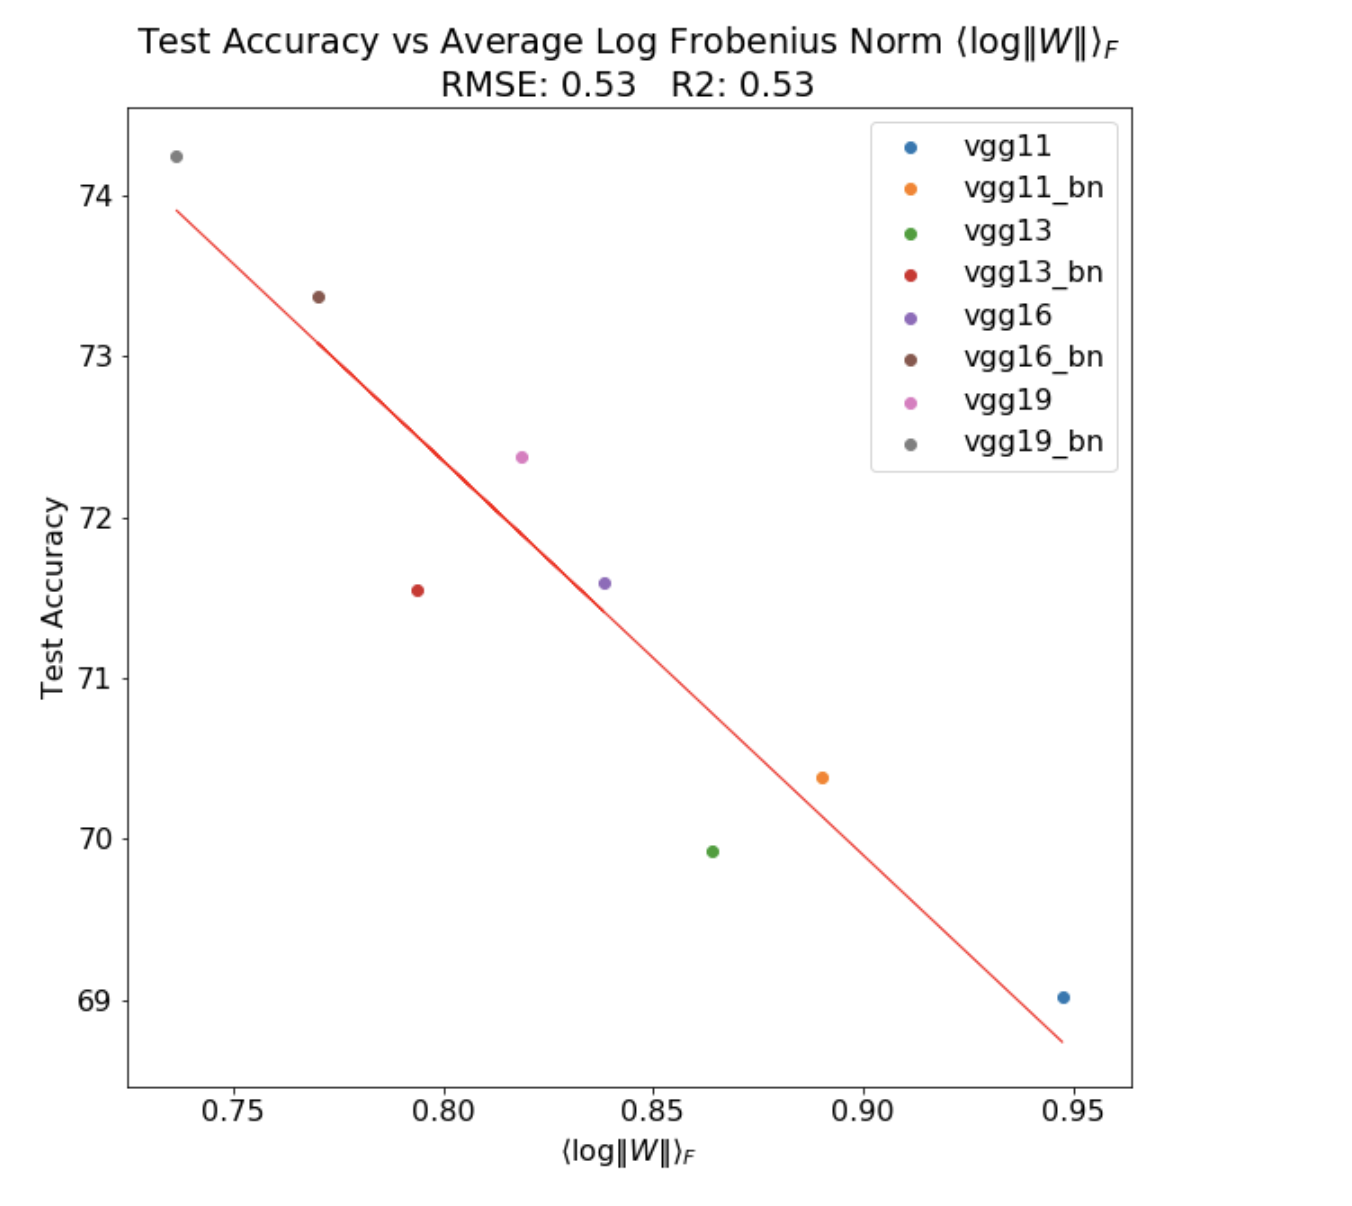
\includegraphics[width=5cm]{img/vgg-fnorm.png}
        \label{fig:vgg-fnorm}
    }
    \qquad
    \subfigure[ Spectral Norm ]{
        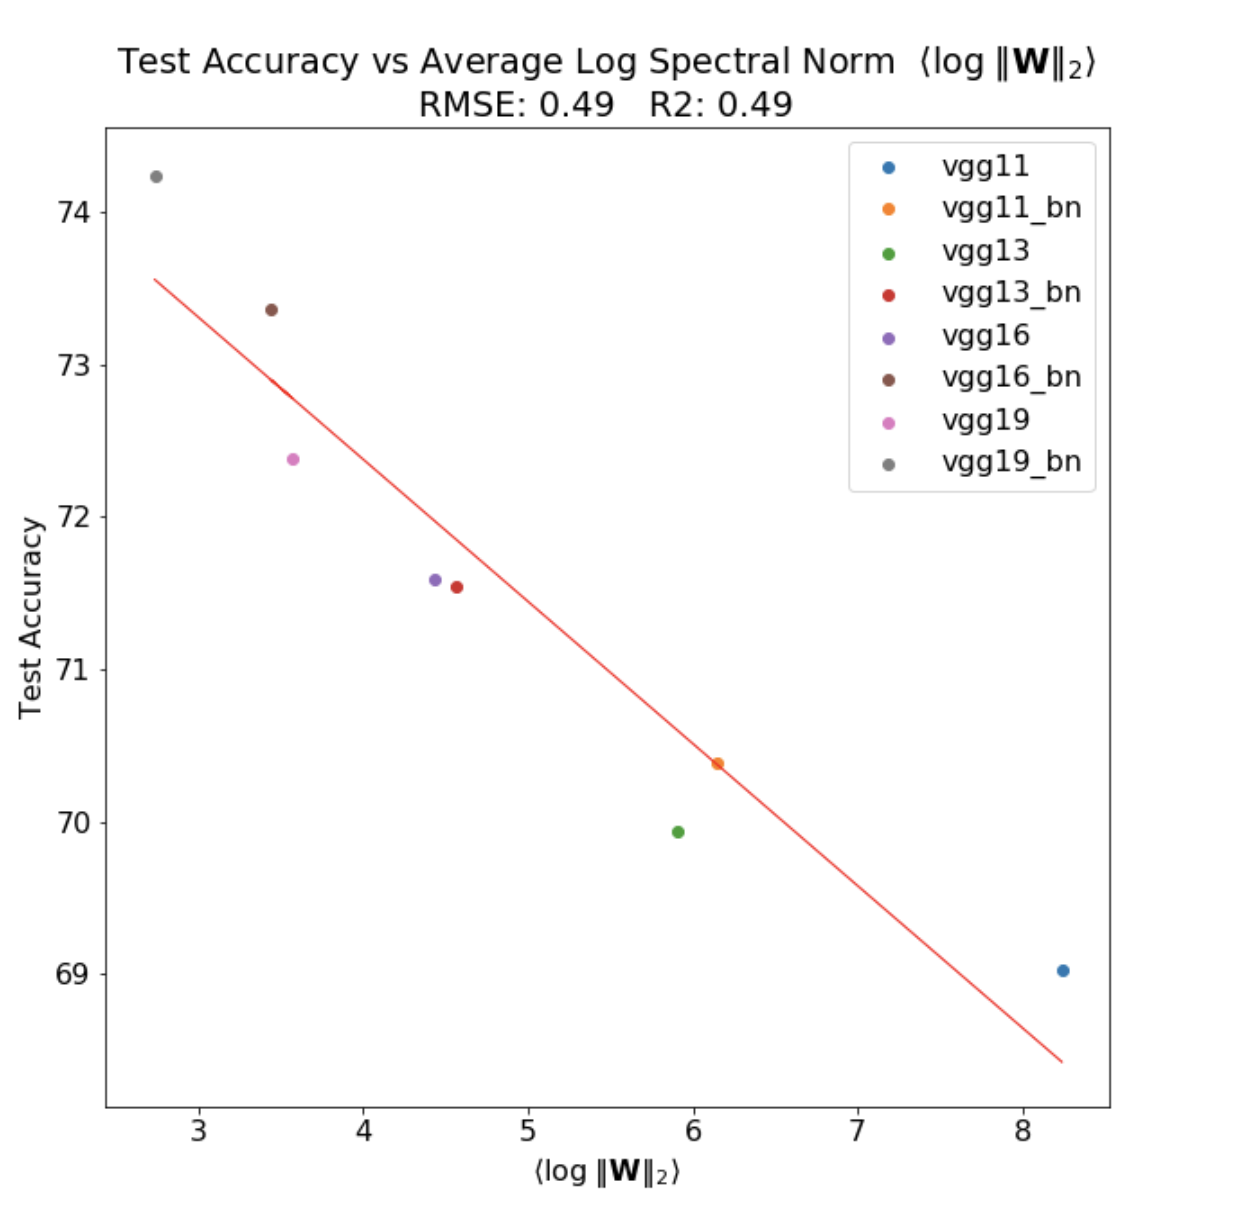
\includegraphics[width=4.9cm]{img/vgg-snorm.png}
        \label{fig:vgg-snorm}
    }
    \qquad
    \subfigure[ Weighted Alpha ]{
        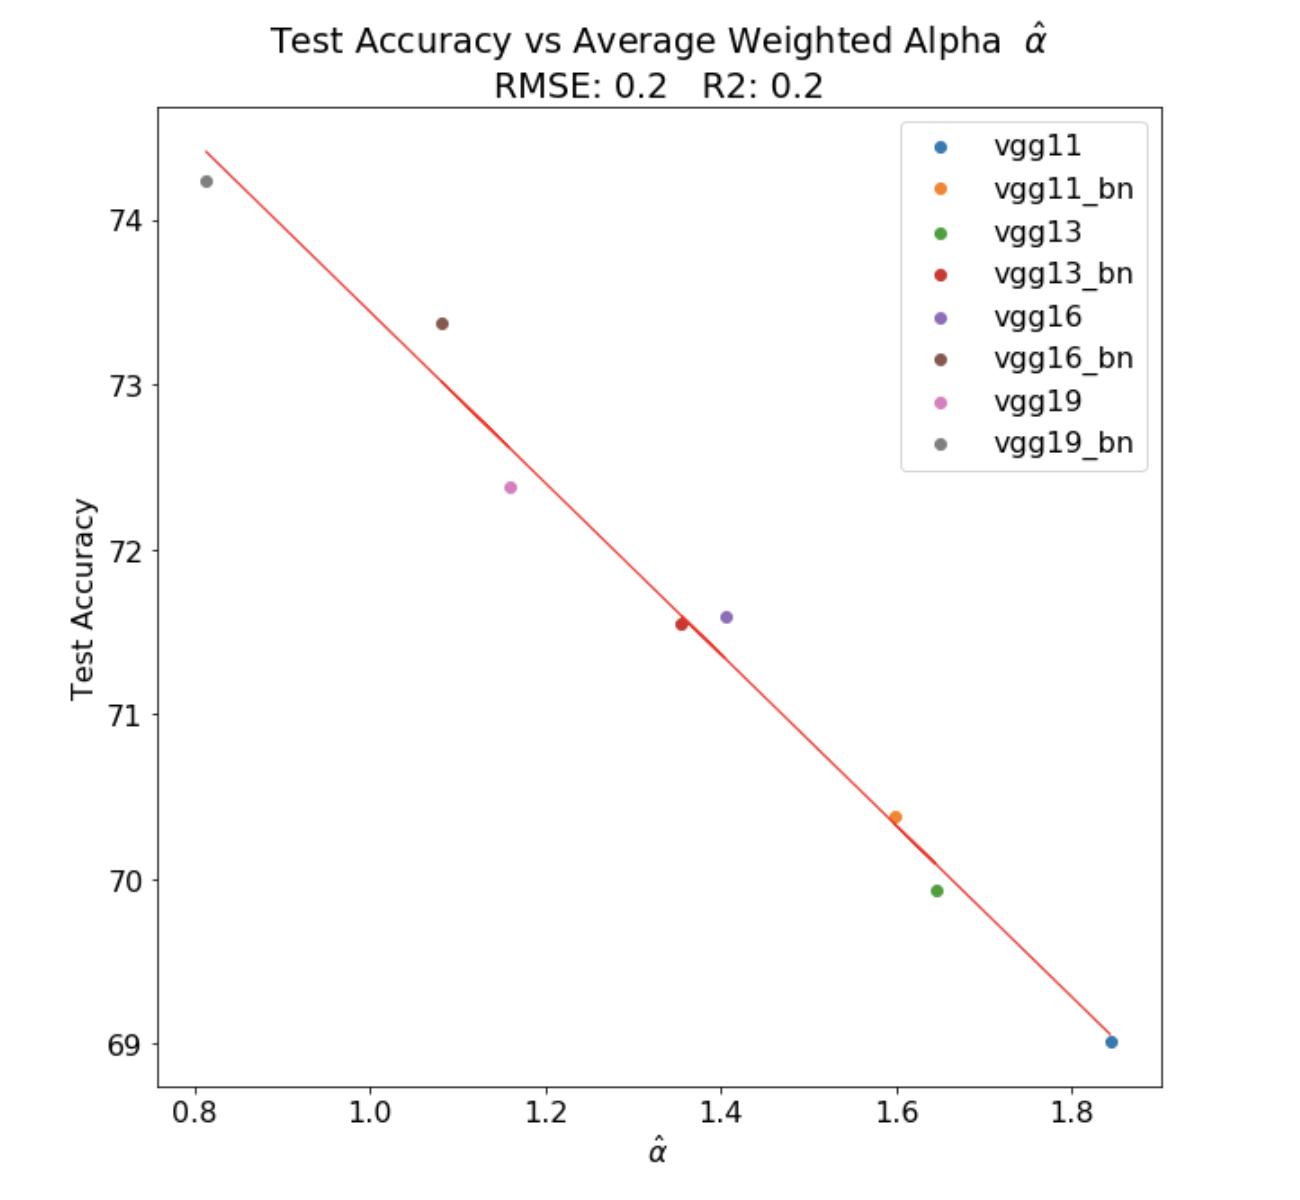
\includegraphics[width=4.9cm]{img/vgg-walpha.png}
        \label{fig:vgg-walpha}
    }
    \qquad
    \subfigure[ Alpha-Norm ]{
        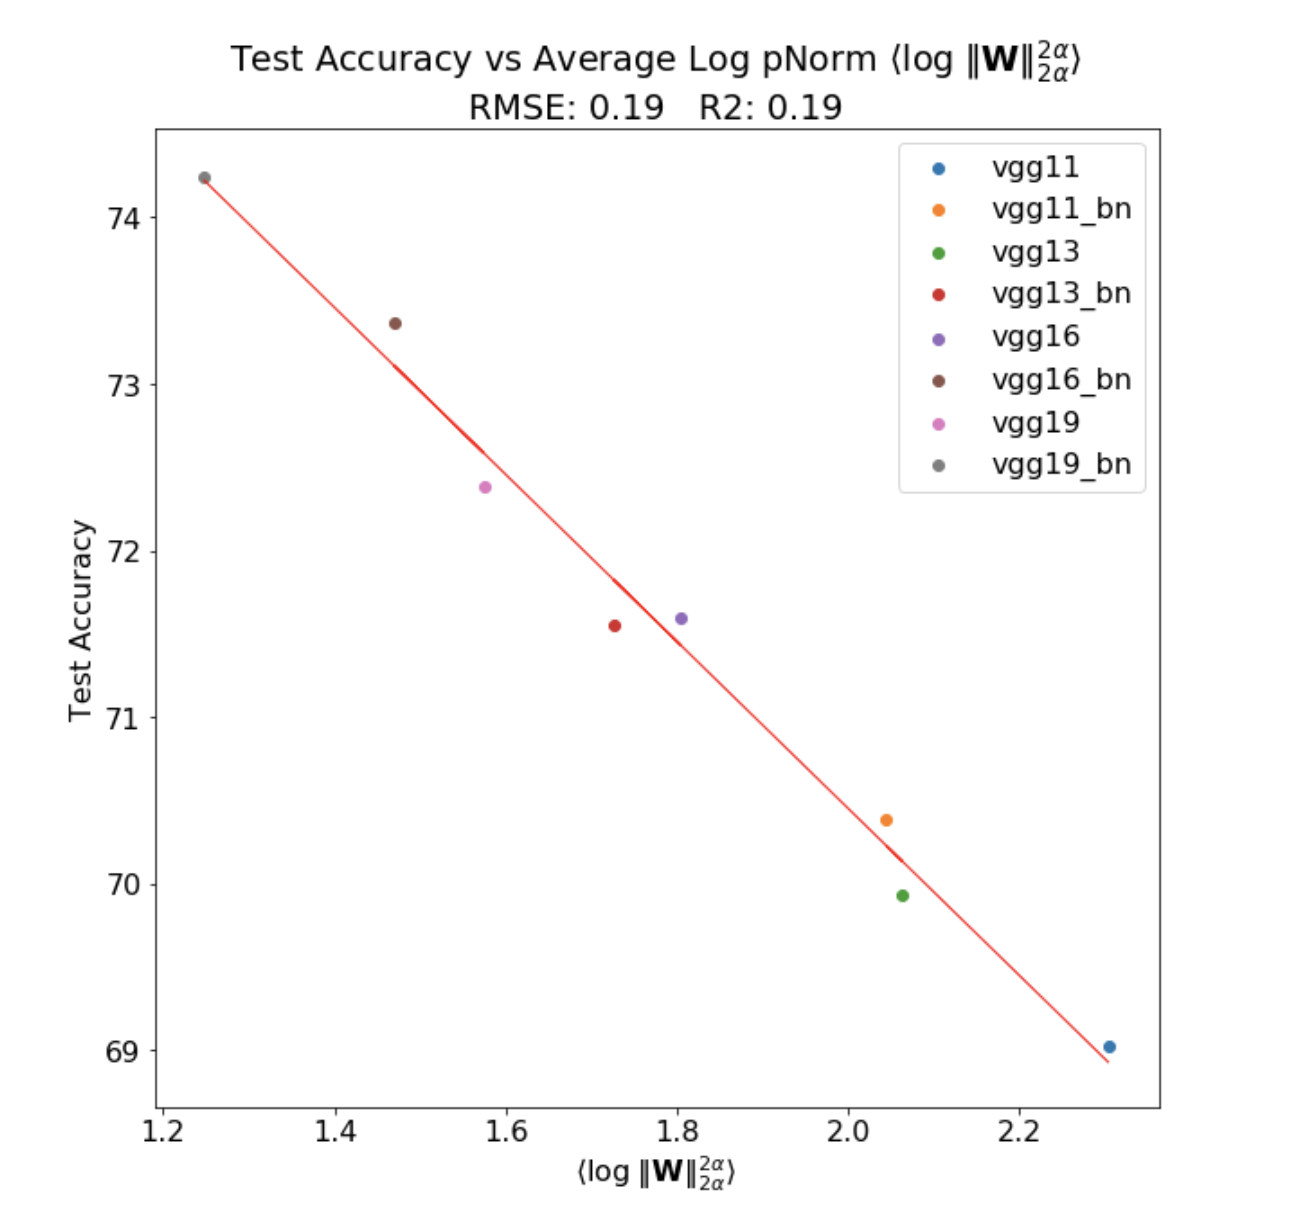
\includegraphics[width=4.9cm]{img/vgg-pnorm.png}
        \label{fig:vgg-pnorm}
    }
    \caption{Comparison of norm metrics vs reported test accuracy for pretrained VGG models, trained on ImageNet, available in pyTorch.  Plots will be updated and replace }
    

    \label{fig:vgg-metrics}
\end{figure}


VGG works remarkably well

ResNet is also correlated, but the RMSE is much larger, and 2/5 of the models are almost outliers
But note that the PyTorch distribution only has a few models.
The ResNet results look better when considering all ResNet models, trained on ImageNet1K.

ADD PLOTS FOR


\begin{figure}[t]
    \centering

    \subfigure[ ResNet ]{
        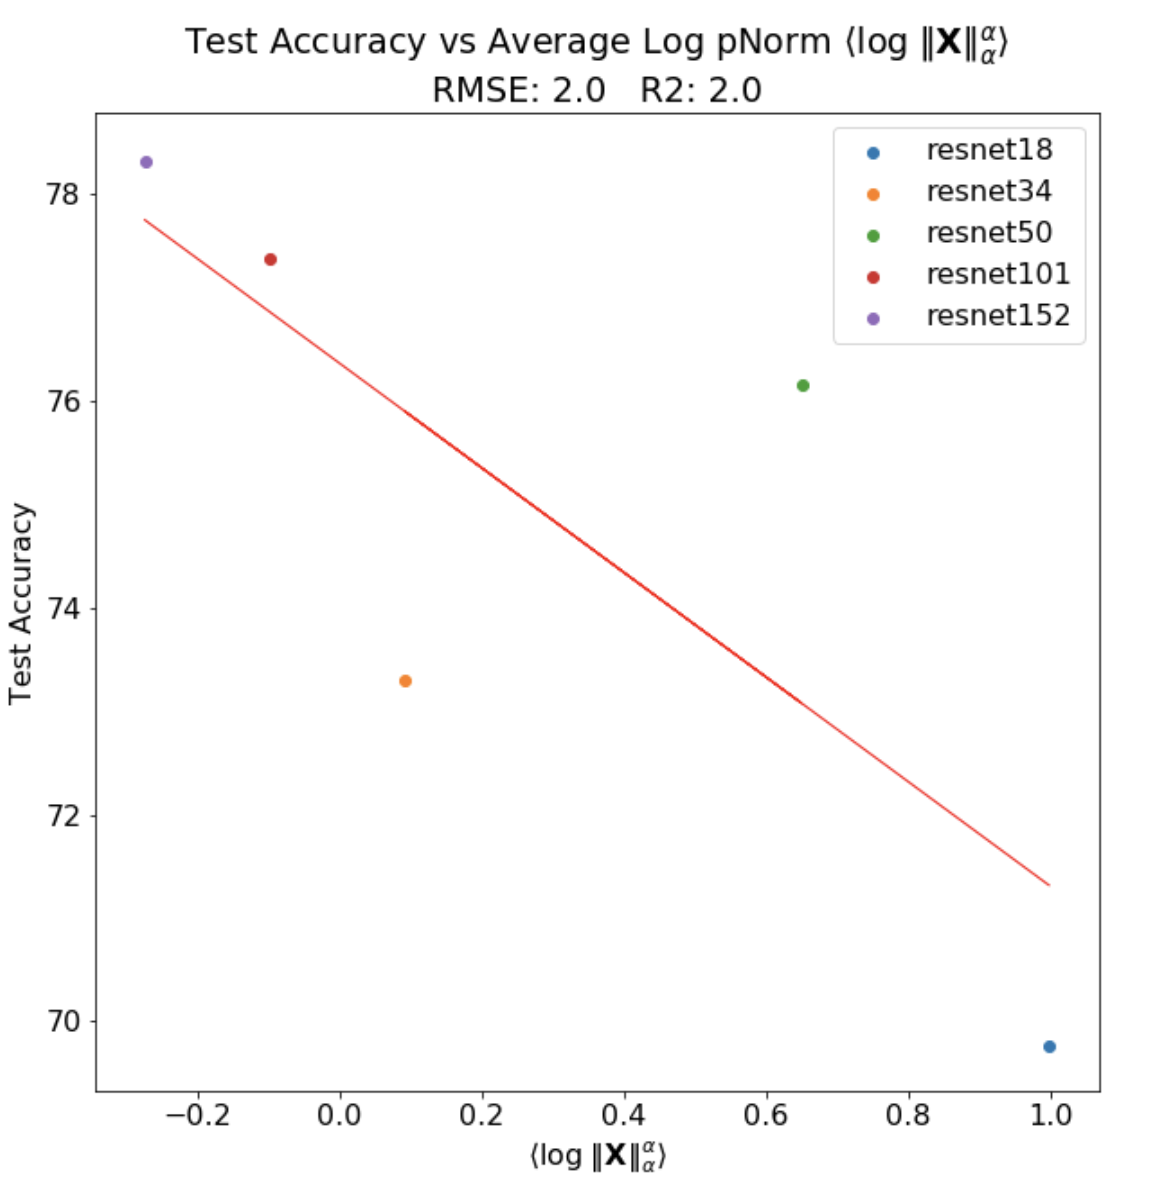
\includegraphics[width=4.2cm]{img/resnet-accuracy.png}
        \label{fig:resnet-accuracy}
    }
    \qquad
    \subfigure[ ResNet-1K ]{
        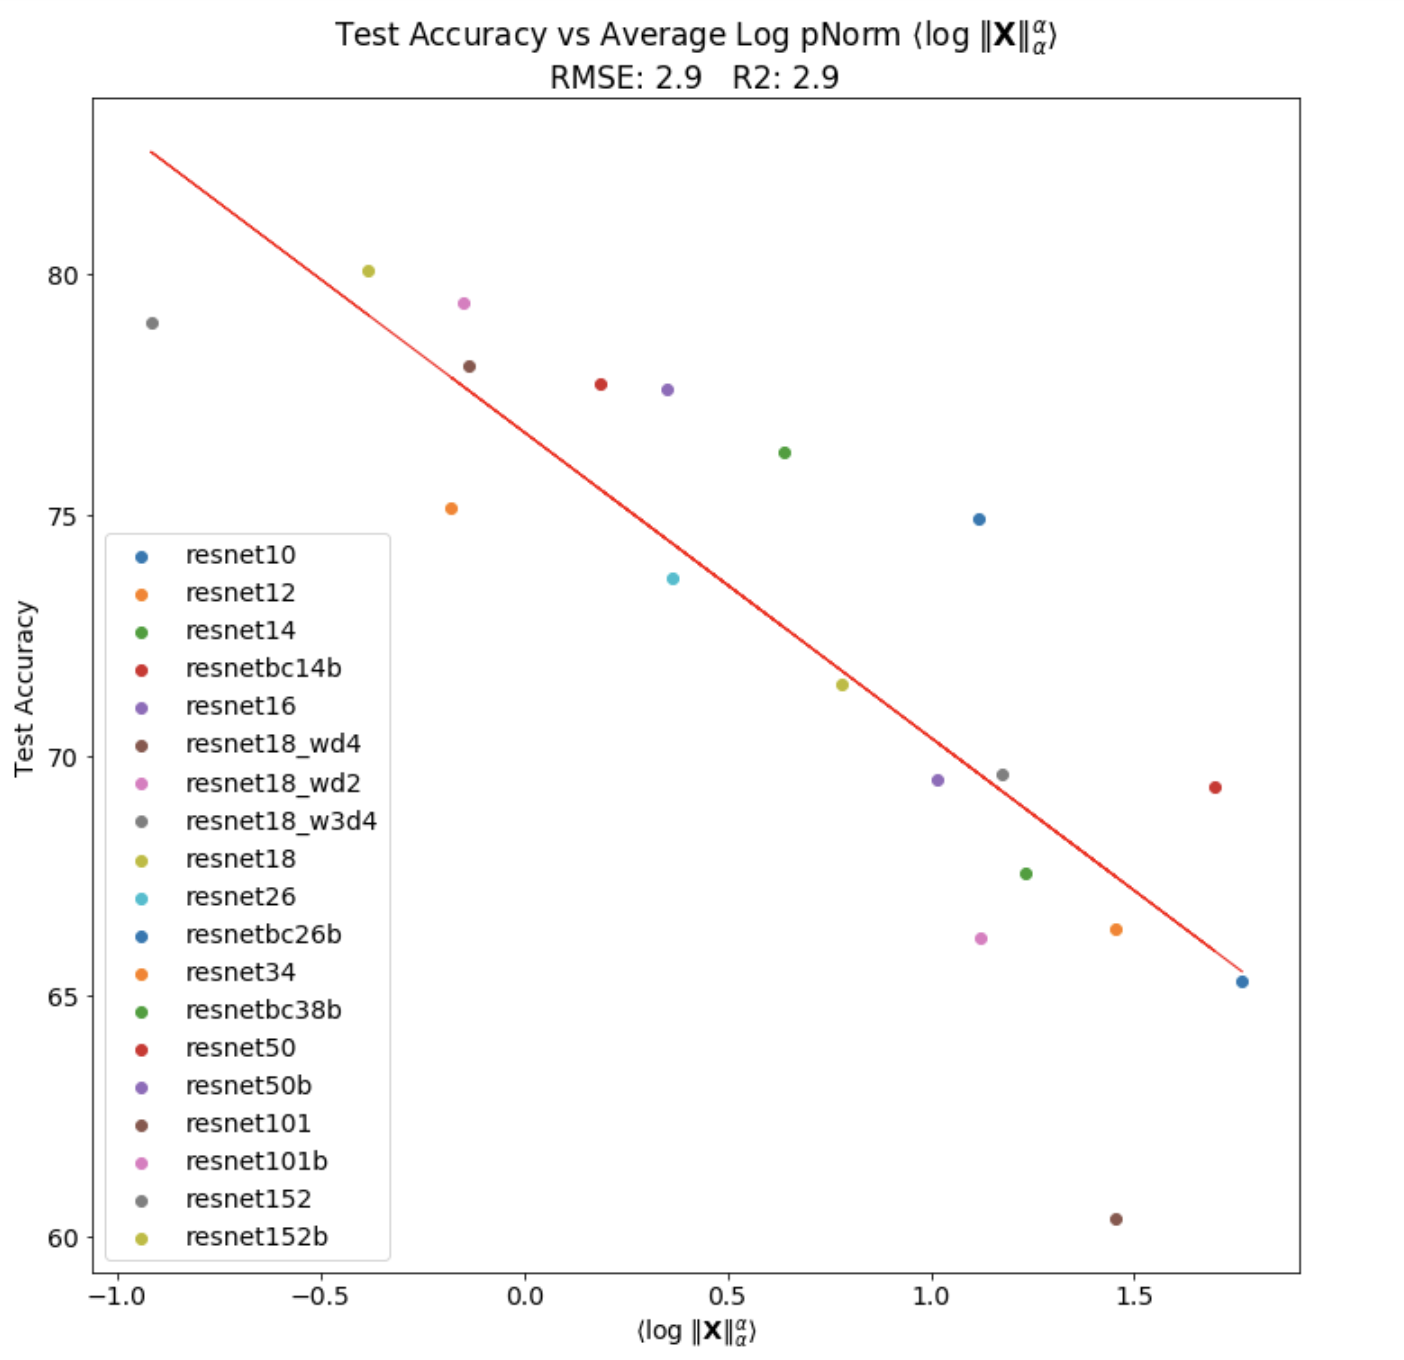
\includegraphics[width=4.5cm]{img/resnet1k-accuracy.png}
        \label{fig:resnet1k-accuracy}
    }
    \qquad
    \subfigure[ DenseNet ]{
        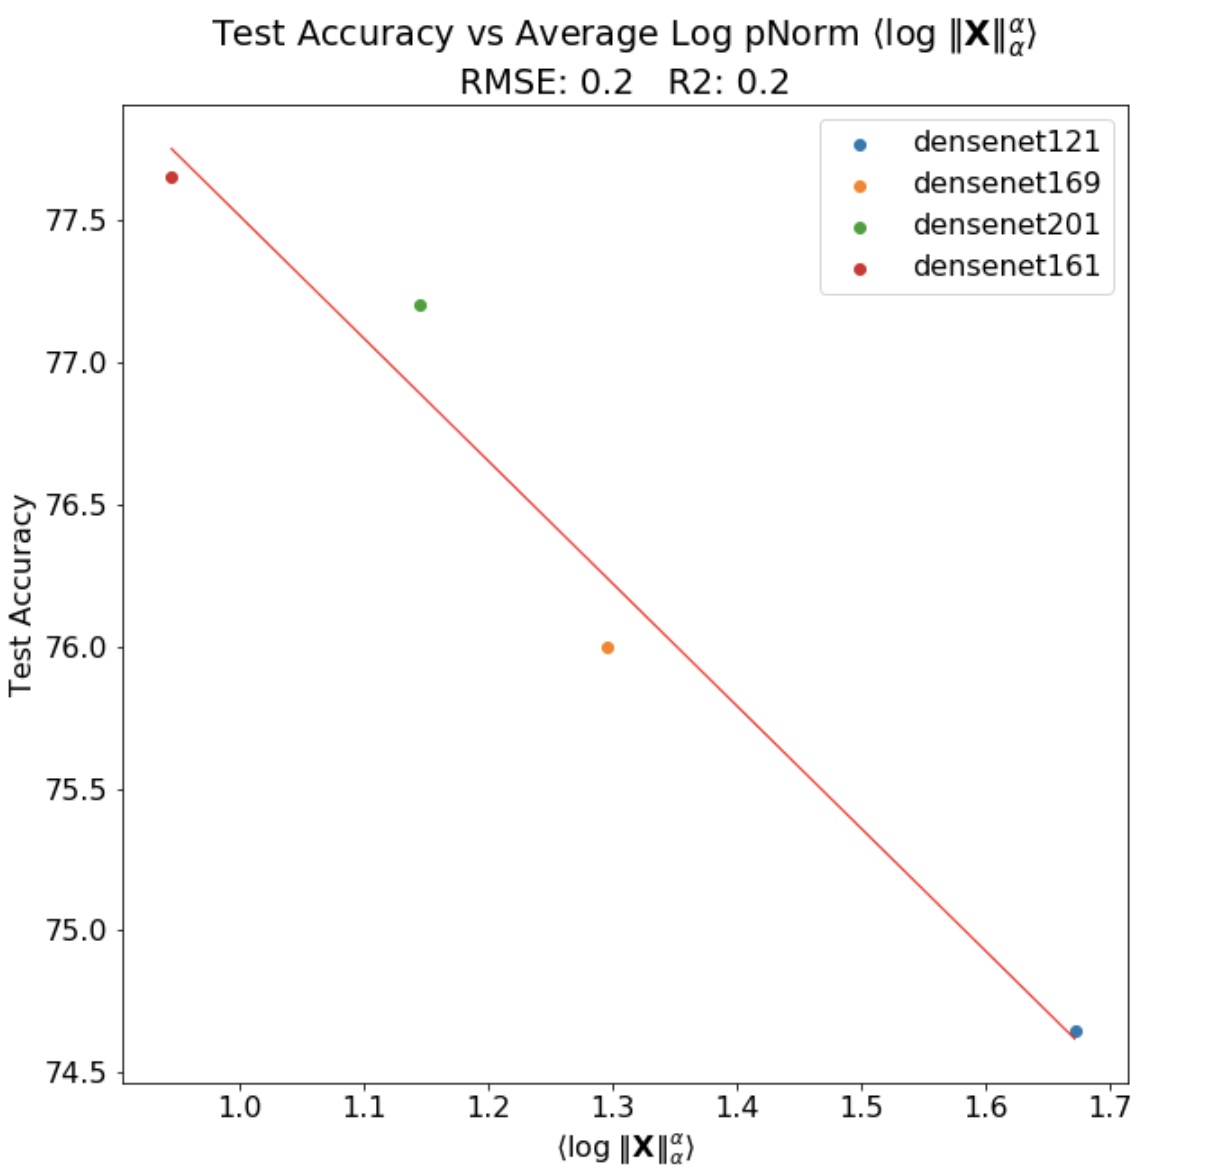
\includegraphics[width=4.4cm]{img/densenet-accuracy.png}
        \label{fig:densenet-accuracy}
    }
    \caption{$\alpha$-Norm vs reported Top1 Error for  ResNet, ResNet-1K, and DenseNet models}
    \label{fig:cv2-accuracy}
\end{figure}


TODO:  add table of metrics for these 3 models, show that alpha-Norm is best again!

\begin{table}[t]
\small
\begin{center}
\begin{tabular}{|p{1in}|c|c|c|c|c|}
\hline
   &    & Frobenius Norm & Spectral Norm & Weighted Alpha & Alpha-Norm \\
 Series & \#Models   & $\Vert\mathbf{W}\Vert_{F}$ & $\Vert\mathbf{W}\Vert_{\infty}$ & $\hat{\alpha}=\alpha\log\lambda_{max}$ & $\Vert\mathbf{X}\Vert^{\alpha}_{\alpha}$ \\
\hline
 VGG & & & & \\
 ResNet & & & & \\
 ResNet-1K & & & & \\
 DenseNet & & & & \\
\hline
\end{tabular}
\end{center}
\caption{RMSE for Linear Fits of Metric to Reported Top1 Test Error for all pre-trained models in the architecture series.  All models trained on ImageNet except ResNet-1K, which was trained on ImageNet-1K. }
\label{table:models}
\end{table}



\paragraph{Correlation Flow in CV Models}

Explain WHAT IS \emph{Correlation Flow}

Compare VGG, ResNet, and DenseNet in the context of how many connections that have

\begin{figure}[t]
    \centering

    \subfigure[ VGG ]{
        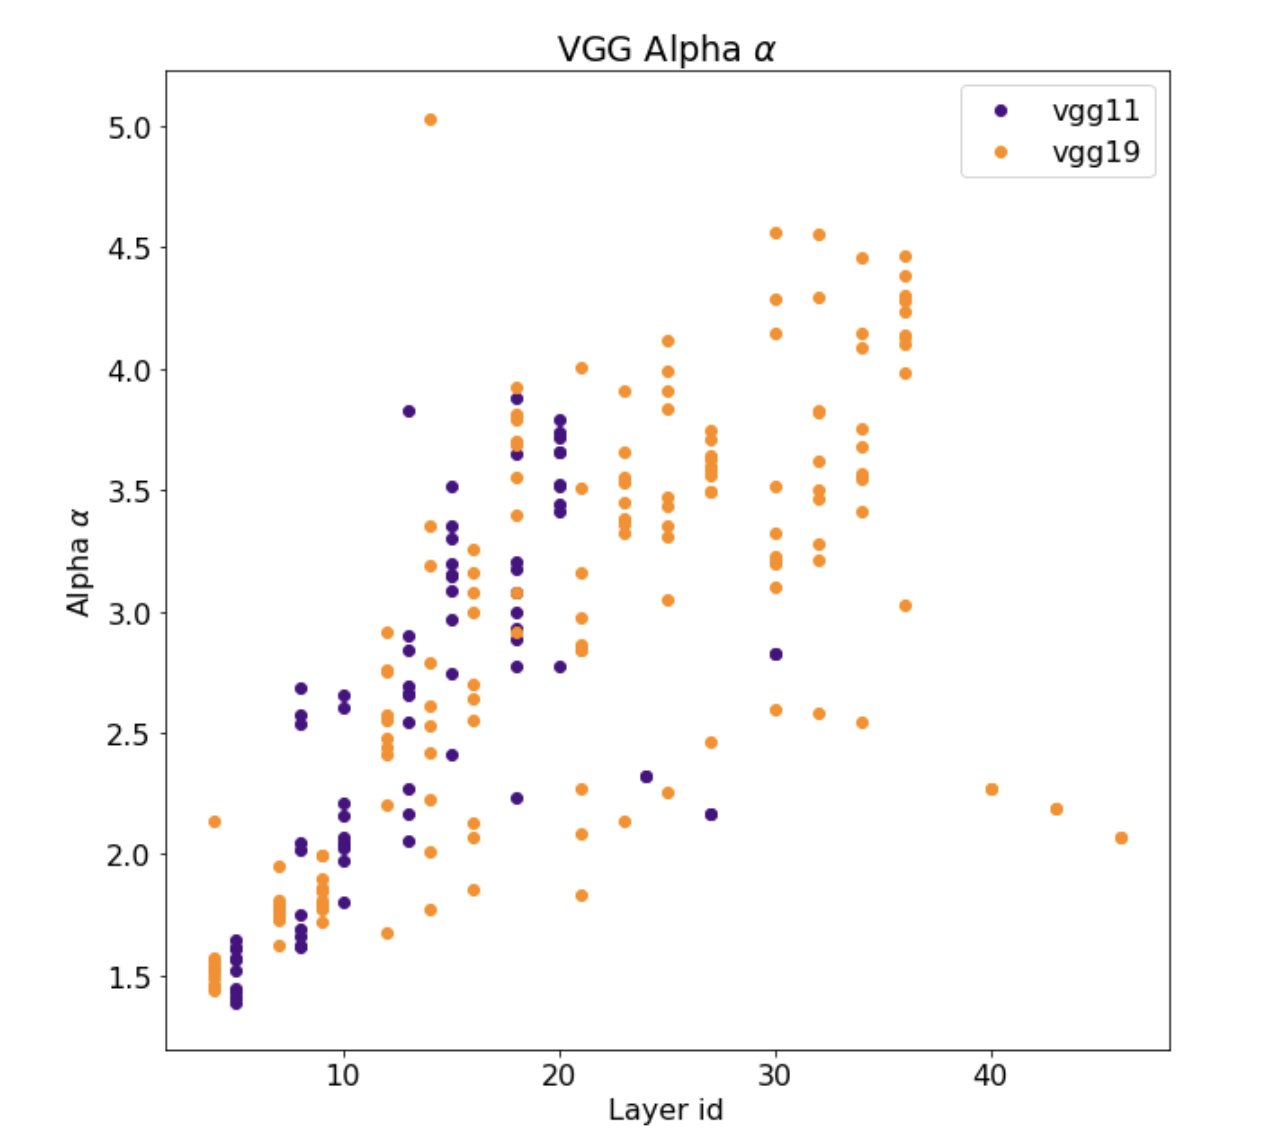
\includegraphics[width=4.1cm]{img/vgg-alpha-layers.png}
        \label{fig:vgg-alpha-layers}
    }
    \qquad
    \subfigure[ ResNet ]{
        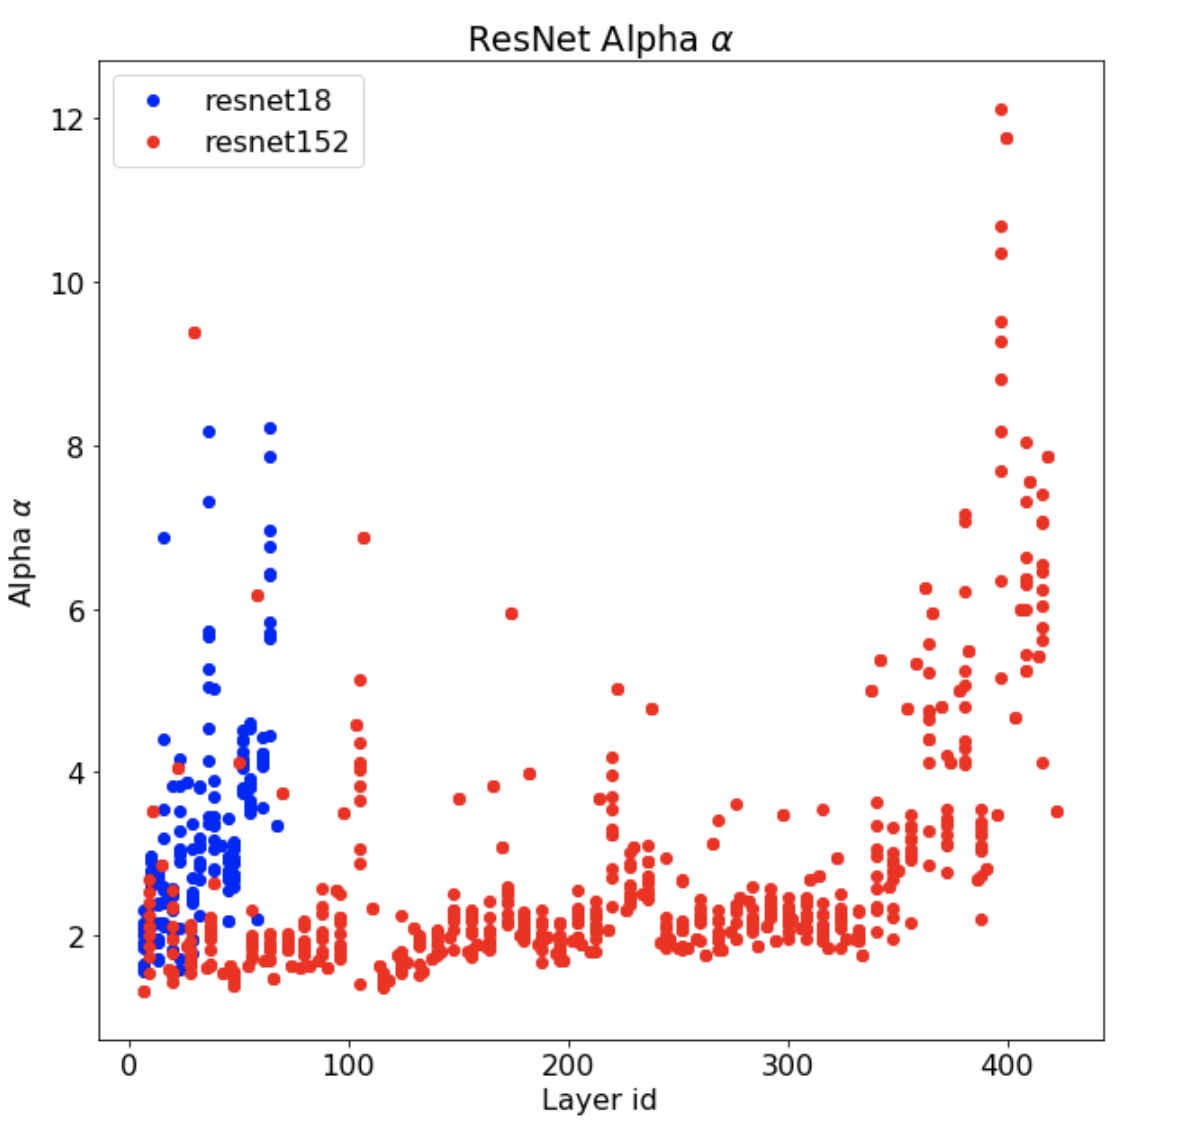
\includegraphics[width=3.8cm]{img/resnet-alpha-layers.png}
        \label{fig:resnet-alpha-layer}
    }
    \qquad
    \subfigure[ DenseNet ]{
        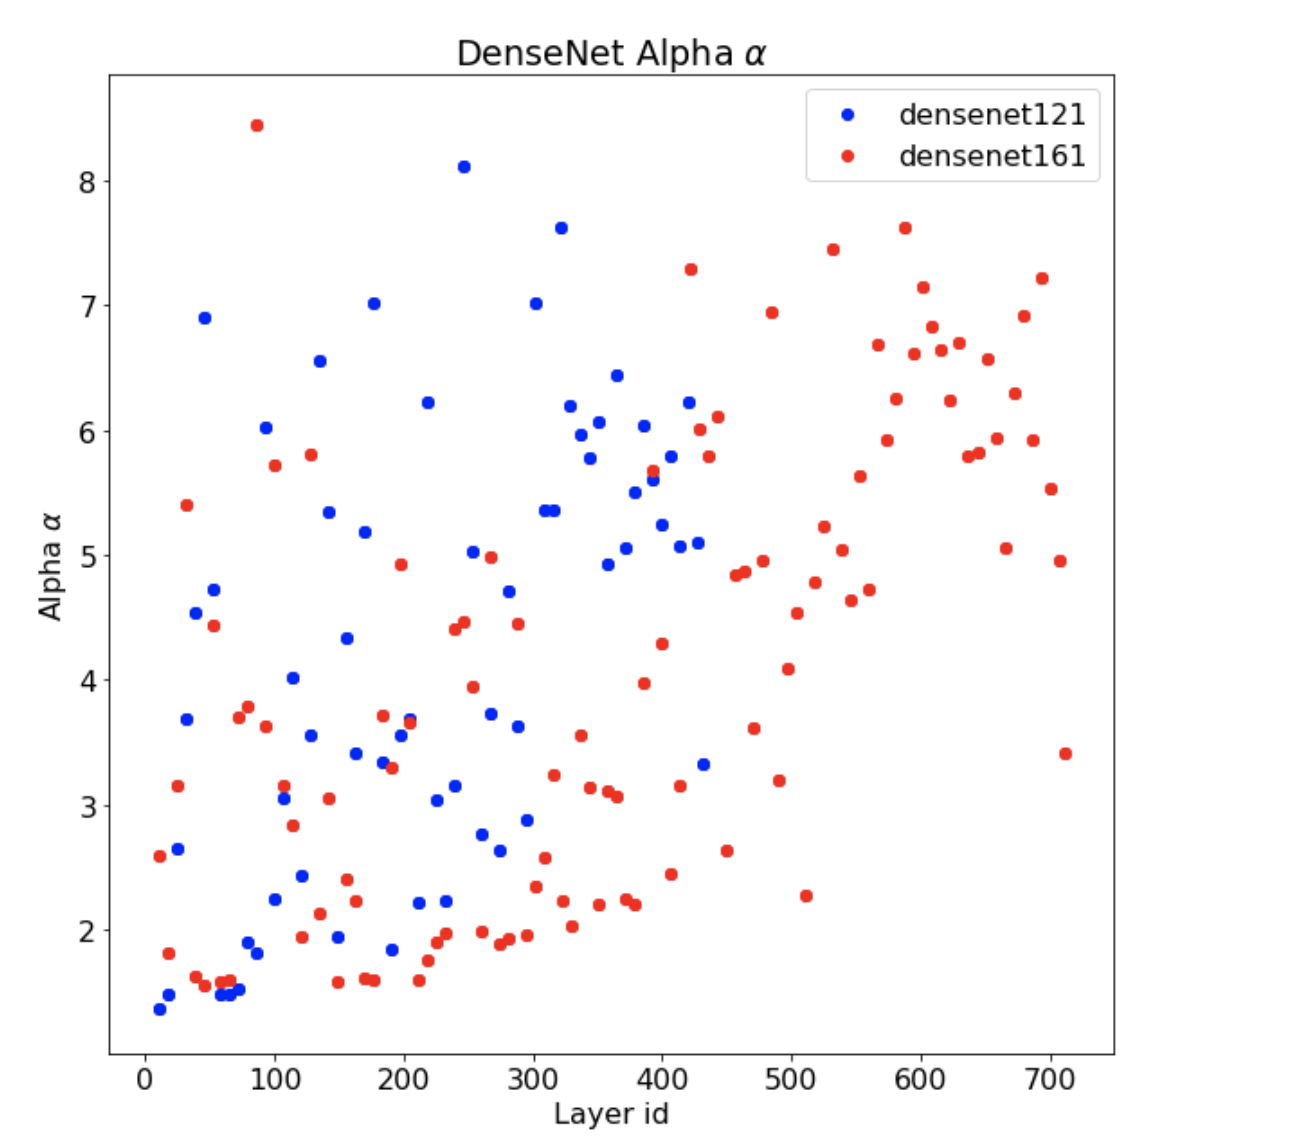
\includegraphics[width=4.1cm]{img/densenet-alpha-layers.png}
        \label{fig:densenet-alpha-layer}
    }
    \caption{Power law exponent $\alpha$ vs layer for VGG, ResNet, and DenseNet models}
    \label{fig:vgg-alpha-layers}
\end{figure}


